The Cox PH model was applied to the Kiddivax data. Subjects were tracked from the start of follow-up to either infection (if they were infected) or end of follow-up (if they were not infected). This analysis assumed that all subjects were followed through a period of similar disease activity and were similarly exposed. The resulting protection curve (relative to the titre of 5) is in Figure \ref{fig:kiddyvaxmain-cox}.

It should be noted that, as demonstrated in the simulation studies, these results may be biased if the assumption that all subjects were similarly exposed is unsatisfied.

\begin{figure}[htp]
    \centering
    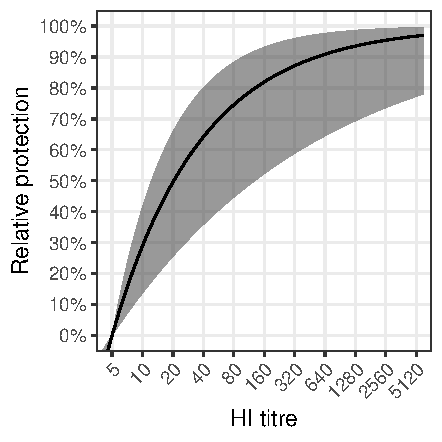
\includegraphics[width=0.5\textwidth]{../fit-cox-plot/kiddyvaxmain-bvic.pdf}
    \caption{
        Fitted relative-to-5 protection curve and confidence interval from the Cox proportional hazards model fit to B Victoria subset of Kiddivax data (shown in Figure \ref{fig:kiddivax-main-summ}). The solid line is the point estimates. The shaded region is the 95\% confidence interval.
    }
    \label{fig:kiddyvaxmain-cox}
\end{figure}
